% Figure: Formalized Mathematics article-to-library link model (story 8).
% Build: pdflatex fm_links.tex  (run inside figures/)
\documentclass[tikz,border=6pt]{standalone}
\usetikzlibrary{positioning,arrows.meta}
\begin{document}
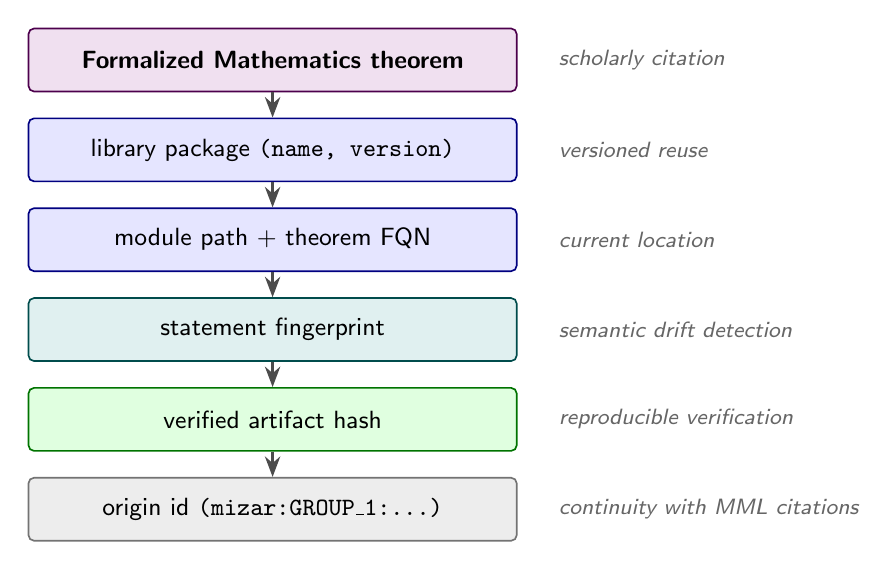
\begin{tikzpicture}[
  font=\sffamily,
  layer/.style={draw, rounded corners=2pt, align=left, minimum width=62mm,
                minimum height=8mm, line width=0.6pt, inner sep=2mm,
                font=\sffamily\small},
  role/.style={font=\sffamily\footnotesize\itshape, text=black!60, align=left,
               anchor=west},
  flow/.style={-{Stealth[length=2.6mm]}, line width=0.9pt, black!70},
  node distance=3.2mm,
]
  \node[layer, fill=violet!12, draw=violet!60!black] (fm)
    {\textbf{Formalized Mathematics theorem}};
  \node[layer, below=of fm, fill=blue!10, draw=blue!50!black] (pkg)
    {library package \texttt{(name, version)}};
  \node[layer, below=of pkg, fill=blue!10, draw=blue!50!black] (fqn)
    {module path + theorem FQN};
  \node[layer, below=of fqn, fill=teal!12, draw=teal!60!black] (fp)
    {statement fingerprint};
  \node[layer, below=of fp, fill=green!12, draw=green!45!black] (hash)
    {verified artifact hash};
  \node[layer, below=of hash, fill=gray!14, draw=black!55] (origin)
    {origin id \texttt{(mizar:GROUP\_1:\dots)}};

  \draw[flow] (fm) -- (pkg);
  \draw[flow] (pkg) -- (fqn);
  \draw[flow] (fqn) -- (fp);
  \draw[flow] (fp) -- (hash);
  \draw[flow] (hash) -- (origin);

  \node[role] at ([xshift=4mm]fm.east)     {scholarly citation};
  \node[role] at ([xshift=4mm]pkg.east)    {versioned reuse};
  \node[role] at ([xshift=4mm]fqn.east)    {current location};
  \node[role] at ([xshift=4mm]fp.east)     {semantic drift detection};
  \node[role] at ([xshift=4mm]hash.east)   {reproducible verification};
  \node[role] at ([xshift=4mm]origin.east) {continuity with MML citations};
\end{tikzpicture}
\end{document}
